\documentclass{article}

% Language setting
% Replace `english' with e.g. `spanish' to change the document language
\usepackage[english, russian]{babel}

% Set page size and margins
% Replace `letterpaper' with `a4paper' for UK/EU standard size
\usepackage[letterpaper,top=1cm,bottom=2cm,left=2cm,right=3cm,marginparwidth=1.75cm]{geometry}

% Useful packages
\usepackage{pdfpages}
\usepackage{amsmath}
\usepackage{algorithm}
\usepackage{algpseudocode}
\usepackage{graphicx}
\newtheorem{theorem}{Определение}
\usepackage[colorlinks=true, allcolors=blue]{hyperref}

\title{Поиск максимальной клики в графе.\\Алгоритм Брона — Кербоша}
\author{Быстров Сергей, Б05-220}
\date{}

\begin{document}
\maketitle

\begin{abstract}
В этом проекта исследуется задача поиска максимальной клики в графе. Основное внимание уделено алгоритму Брона — Кербоша, который позволяет перечислить все максимальные клики в графе. Была рассмотрена как базовая версия алгоритма, так и его две модификации, позволяющие добиться существенных ускорений на практике. Описаны принципы работы алгоритма, его сложность.

В практической части было произведено сравнение базового алгоритм и его улучшенной версии на разных типах графов: случайных, полных и графах Турана. Была продемонстрирована эффективность улучшенной версии алгоритма. 

\end{abstract}
\newpage

\tableofcontents

\newpage
\section{Введение}
Как известно, задача о поиске максимальной клики является NP-полной.
\begin{theorem}
Клика, которая не содержится в клике большего
размера, называется максимальной кликой.
\end{theorem}
В рамках данного проекта мы рассмотрим задачу нахождения \textbf{всех} максимальных клик в графе. Пока что нам только известно, что эта задача лежит в $EXP$, тем самым является более сложной версией исходной. В рамках данного проекта мы рассмотрим алгоритм Брона — Кербоша, имеющий асимптотику $$\mathcal{O}(\#\text{количество клик максимального размера})=\mathcal{O}(3^\frac{n}{3})$$
где $n$ - количество вершин в графе.\\\\
Так как асимптотика зависит именно от \textit{количества максимальных клик}, то на практике алгоритм Брона — Кербоша часто оказывается эффективным решением. В совокупности с простотой реализации, этот алгоритм до сих пор используется как для решения задачи поиска максимальной клики, так и нахождения всех максимальных клик.

\textbf{Актуальность} данной работы заключается в том, что нахождение максимальных клик в графах имеет важное практическое значение в таких областях, как биоинформатика, анализ социальных сетей, обработка данных и безопасность. Нахождение клик помогает выделять важные группы объектов с сильными взаимными связями. Алгоритм Брона — Кербоша, предложенный ещё в 1973 году, несмотря на то что существует очень давно, продолжает оставаться актуальным и используется в различных областях, поэтому его изучение представляет большой инетерс.


\newpage
\section{Теоретическая часть}
\subsection{Используемые понятия и обозначения}
В рамках данного проекта будем рассматривать \textit{неориентированные графы}.
\begin{theorem}
Графом \textbf{\( G \)} называется пара \( G = (V, E) \), где \( V \) — это конечное множество вершин, а \( E \) — это множество рёбер, каждое из которых является парой элементов из множества \( V \). Рёбра могут быть ориентированными или неориентированными, в зависимости от типа графа.
\end{theorem}

\begin{theorem}
Неориентированным графом \( G = (V, E) \) называется граф, в котором рёбра не имеют направления, то есть для любого ребра \( e = (u, v) \in E \) выполняется \( (u, v) = (v, u) \). 
\end{theorem}

При изучении алгоритма Брона - Кербоша нам понадобится следующее понятие:

\begin{theorem}
Соседями вершины \( v \in V \) в графе \( G = (V, E) \) называются все вершины \( u \in V \), такие что существует ребро \( e = (v, u) \in E \). Множество соседей вершины \( v \) обозначается \( N(v) \), то есть \( N(v) = \{ u \in V : (v, u) \in E \} \).
\end{theorem}

Для тестирования алгоритма нас будут интересовать конкретные графы, а именно:
\begin{theorem}
Полный граф \( K_n \) — это граф, состоящий из \( n \) вершин, в котором каждая пара различных вершин соединена ровно одним ребром. Формально, \( E(K_n) = \{ (u, v) : u, v \in V, u \neq v \} \).
\end{theorem}

\begin{theorem}
Случайный граф \( G(n, p) \) — это граф с \( n \) вершинами, в котором каждое возможное ребро между парой вершин существует с независимой вероятностью \( p \), где \( 0 \leq p \leq 1 \). Формально, для каждой пары вершин \( u, v \) вероятность того, что рёбер \( (u, v) \) существует, равна \( p \).
\end{theorem}

\begin{theorem}
Граф Турана $T(n,r)$ — это граф, образованный разложением $n$ вершин на $r$ подмножеств, с как можно близким размером, и вершины в этом графе соединены ребром, если они принадлежат разным подмножествам
\end{theorem} \newline

\subsection{История задачи поиска максимальной клики}

Задача о поиске полных подграфах впервые подробно изучается в середине $20$ века.

\textbf{1935:} Полные подграфы (которые позже будут названы кликами) были впервые рассмотрены в теоретико-графовой формулировке в контексте теории Рамсея, разработанной Эрдишем и Секерешем. Эта теория изучала математические свойства графов, где важно наличие полных подграфов.\\
\textbf{1949:} Люс и Перри использовали графы для моделирования социальных сетей и адаптировали терминологию социальных наук к теории графов. Именно они ввели термин "клика", обозначая этим полные подграфы, которые используются для описания групп людей, знакомых друг с другом.\\\\
Изучение же алгоритмов поиска максимальных клик началось в $70$-х годах.

\textbf{1970-е годы}: Исследования алгоритмов для поиска кликов стали более систематическими. В 1977 году Тарджан и Трояновский изучили сложность задачи поиска максимальной клики с точки зрения анализа наихудшего случая.
В это же время начались работы, посвящённые применению теории NP-полноты для объяснения сложности задачи. В \textbf{1971} году Кук, а в \textbf{1972} году Карп предложили первые результаты, которые математически доказали, что задача поиска максимальной клики является NP-полной.

\textbf{1991}: Исследования Файга и коллег показали, что задача поиска максимальной клики является не только NP-полной, но и трудно приближаемой. Это открытие установило, что нет эффективных алгоритмов для решения этой задачи, даже с приближёнными решениями, если не доказано $P \neq NP$.

В таблице \ref{tab:clique_algorithms} представлена история создания алгоритмов для поиска максимальной клики в графе.
\begin{table}[h!]
\centering
\begin{tabular}{|c|c|c|c|}
\hline
\textbf{Год} & \textbf{Авторы} & \textbf{Алгоритм} & \textbf{Асимптотика} \\ \hline
1973 & Брон, Кербош & Алгоритм Брона — Кербоша & \( O(3^{n/3}) \) \\ \hline
1977 & Тарджан, Трояновский & Алгоритм для анализа наихудшего случая & \( O(2^{n/3}) \) \\ \hline
1986 & Цзянь & Улучшенная версия алгоритма Тарджана и Трояновского & \( O(2^{0.304n}) \) \\ \hline
1986 & Робсон & Алгоритм Робсона & \( O(2^{0.276n}) \) \\ \hline
2001 & Робсон & Усиленная версия алгоритма Робсона & \( O(2^{0.249n}) \) \\ \hline
\end{tabular}
\caption{Алгоритмы для поиска максимальной клики}
\label{tab:clique_algorithms}
\end{table}

\subsection{Базовая версия алгоритма Брона Кербоша}
Алгоритм строит клики в графе итерационно, полагаясь на тот факт, что каждая клика уже является максимальной по включению. Он начинает с одиночной вершины и на каждом шаге пытается расширить текущий полный подграф, выбирая вершины из \textit{списка кандидатов}. Отдельным множеством алгоритм передаются вершины, которые уже точно не приведут к созданию клики. Таким образом в алгоритме задействованы три множества:

• множество, содержащее полный подграф на каждом шаге поиска ($R$)

• множество вершин, которые могут быть добавлены в первое множетсво для расширения подграфа($P$)

• множество вершин, которые уже были использованы для расширения первого множества на предыдущих шагах поиска ($X$)

Таким образом, базовая версия алгоритм  выглядит следующим образом:

\begin{algorithm}
\caption{Алгоритм Брона — Кербоша}
\begin{algorithmic}[1]
\Procedure{BronKerbosch1}{$R, P, X$}
    \If{$P$ и $X$ обе пусты}
        \State \texttt{return} $R$ как максимальную клику
    \EndIf
    \For{каждая вершина $v$ в $P$}
        \State \Call{BronKerbosch1}{$R \cup \{v\}, P \cap N(v), X \cap N(v)$}
        \State $P := P \setminus \{v\}$
        \State $X := X \cup \{v\}$
    \EndFor
\EndProcedure
\end{algorithmic}
\end{algorithm}

Базовая форма алгоритма, описанная выше, неэффективна в случае графов с множеством немаксимальных клик: он делает рекурсивный вызов для каждой клики, и неважно максимальной или нет. Следующие две вариации этого алгоритма избавляются от лишних рекурсий. Первый выбирает "поворотную вершину" из P, соседи которой не будут проверяться на нахождение в максимальной клики, второй задает специальный порядок на вершинах, обход которого позволяет убрать лишние итерации.


\subsection{Первое улучшение: with pivoting}
Рассмотрим подробнее первое улучшение: выбор опорной точки. Чтобы сэкономить время и позволить алгоритму быстрее возвращаться из ситуаций, которые не содержат максимальных клик, Брон и Кербош представили \cite{Bron1973} вариант алгоритма, включающий "поворотную вершину" u, выбранную из P. Cоседи этого опорного элемента не проверяются рекурсивно. Любая максимальная клика, потенциально найденная в тестах соседей u, также будет найдена при тестировании u или одного из его несоседей, поскольку хотя бы один из них всегда будет частью этой максимальной клики. В противном случае только соседи u были бы частью этой максимальной клики, что позволяло бы увеличить ее путем добавления к ней u что противоречит тому, что эта клика является максимальной. Следовательно, только u и ее не-соседей необходимо проверять в качестве выбора вершины v, которая добавляется к R при каждом рекурсивном вызове алгоритма.

\begin{algorithm}
\caption{Алгоритм Брона — Кербоша с опорной вершиной (Bron-Kerbosch2)}
\label{alg:bronkerbosch2}
\begin{algorithmic}[1]
\Procedure{BronKerbosch2}{$R, P, X$}
    \If{$P = \emptyset$ \textbf{and} $X = \emptyset$}
        \State \textbf{report} $R$ \Comment{Нашли максимальную клику}
    \EndIf
    \State Выбрать опорную вершину $u$ из $P \cup X$
    \For{\textbf{each} $v \in P \setminus N(u)$}
        \State \Call{BronKerbosch2}{$R \cup \{v\}, P \cap N(v), X \cap N(v)$}
        \State $P \gets P \setminus \{v\}$
        \State $X \gets X \cup \{v\}$
    \EndFor
\EndProcedure
\end{algorithmic}
\end{algorithm}

\subsection{Второе улучшение: with vertex ordering}

Альтернативный метод улучшения базовой версии алгоритма Брона — Кербоша заключается в отказе от выбора опорной вершины на самом внешнем уровне рекурсии. Вместо этого тщательно выбирается порядок рекурсивных вызовов с целью минимизации размеров множеств \( P \) кандидатов в вершины на каждом уровне рекурсии.

\begin{theorem}
Вырожденность графа \( G \) определяется как минимальное число \( d \), такое что любой подграф графа \( G \) содержит вершину со степенью не больше \( d \).
\end{theorem}

Для любого графа можно построить порядок вырожденности — порядок вершин, при котором каждая вершина имеет не более \( d \) соседей, идущих позже в этом порядке. Такой порядок можно найти за линейное время, последовательно выбирая вершину с минимальной степенью среди оставшихся вершин.

Если порядок вершин \( v \), по которым выполняется цикл в алгоритме Брона — Кербоша, соответствует порядку вырожденности, то множество \( P \) (кандидатов в вершины для текущего рекурсивного вызова) будет гарантированно иметь размер не больше \( d \) (соседи \( v \), которые идут позже в порядке). Множество \( X \) (исключённых вершин) будет содержать всех соседей \( v \), идущих раньше, и может быть гораздо больше \( d \). На уровнях рекурсии ниже верхнего уровня можно по-прежнему использовать версию алгоритма с опорной вершиной.

\begin{algorithm}
\caption{Алгоритм Брона — Кербоша с порядком вырожденности (Bron-Kerbosch3)}
\label{alg:bronkerbosch3}
\begin{algorithmic}[1]
\Procedure{BronKerbosch3}{$G$}
    \State $P \gets V(G)$
    \State $R \gets \emptyset, X \gets \emptyset$
    \For{\textbf{each} вершина $v$ в порядке вырожденности графа $G$}
        \State \Call{BronKerbosch2}{$\{v\}, P \cap N(v), X \cap N(v)$}
        \State $P \gets P \setminus \{v\}$
        \State $X \gets X \cup \{v\}$
    \EndFor
\EndProcedure
\end{algorithmic}
\end{algorithm}

\subsection{Корректность}

1. Алгоритм распознает только максимальные клики. Действительно, мы начинаем в вершине - клики. На каждом из следующих шагов мы получаем только клики, так как во множестве $P$ остаются только вершины, имеющие ребра со всеми вершинами из множества $X$ \\\\
2. Мы находим все максимальные клики. Действительно, так как мы начинаем во всех вершинах, то в том числе и в вершине, находящейся в рассматриваемой клики. На каждом этапе, мы получаем клику, завершаемся когда не остается вершин, соединенных со всеми вершинами из нашего множества $X$, то есть когда клику нельзя расширить, то есть когда достигли максимальную клику.

\subsection{Асимптотика}
В случае удачно выбранных pivot-вершин для второго варианта алгоритма количество итераций ограничено количеством максимальных клик. Аналогична ситуация и для третьего варианта. Эти нетривиальные факты приведены и доказываются в \cite{Bron1973} и \cite{Tomita2006} соответственно. Мы же покажем, что число максимальных клик есть $\mathcal{O}(3^\frac{n}{3})$ (теорема Moon и Moser (1965) \cite{Moon1965}), тем самым покажем, что асимптотика улучшенных версий алгоритм $\mathcal{O}(3^\frac{n}{3})$

Jбозначим через $f(n)$ количество максимальных клик
$n \ge 2$, тогда
\begin{equation*}
f(n) = 
 \begin{cases}
   $3^{\frac{n}{3}}$ &\text{$ n\equiv 0 \mod 3$}\\
   $4.3^{\frac{n}{3} - 1}$ &\text{$ n\equiv 1 \mod 3$}\\
   $2.3^{\frac{n}{3}}$ &\text{$ n\equiv 2 \mod 3$}
 \end{cases}
\end{equation*}
Нетрудно проверить это при $n = 2$ (клика размера 2), для 3, 4 аналогично. Тогда стоит рассмотреть графы при $n >= 5$ (допустим, граф связен) и обозначим количество клик в графе череp $c(G)$. Смежные вершины обозначим через Г$(x)$.

Через $\alpha(x)$ обозначим количество графов, содержащихся в Г$(x)$, являющихся максимальными по отношению к $G/${x}.

Через $\beta(x)$ обозначим количество графов, содержащихся в Г$(x)$, являющихся максимальными по отношению к Г$(x)$, но не $G/${x}. Заметим, что $\beta(x, y) = \beta(y, x)$

Тогда также очевидно, что $c(G/x) = c(G) - \beta(x)$. Обозначим за $\chi(x)$ число клик в G, содержащих x.

Так как $\alpha(x)$ и $\beta(x)$ дополняют друг друга и не пересекаются, то $\chi(x) =\alpha(x) + \beta(x)$.

Рассмотрим две несвязанные вершины в графе G: x и y. Обозначим через G(x,y) такой граф, что связанные с x ребра удаляются и заменяются ребрами, соединяющие x с каждой вершиной Г($y$).

$c(G(x, y)) = c(G) + \chi(y) - \chi(x) + \alpha(x)$.

Пусть G - любой граф, у которого $n >= 5$ вершин, а также максимальное количество клик. G связан, ни одна вершина не связана с каждой оставшейся.

$\chi(y) > \chi(x)$ => G(x,y) был бы более выгодным по количеству клик, а потому в нашем графе G: $\chi(y) = \chi(x)$. \forall x \in G $\alpha(x) = 0$. $G^{1} = G$ (это обозначение, позже мы используем G с индексами).

Возьмем произвольную вершину x \in G и обозначим за a, b, c, d, e, f не связанные с ней вершины. $G^{2} = G(a, x)$. Заменим теперь $G^{1}$ на $G^{2}$, потому что это не влияет на количество и размер максимальной клики. Заменяем далее $G^{2}$ на $G^{3}$ и так далее. После всех замен получим граф с теми же свойствами, но x, a, ... f не будут связаны между собой, при этой связаны с остальными. Теперь применим ту же процедуру к вершине y в Г($x$). Получили итоговый граф G, такой что мы можем разделить вершины на непересекающиеся множества по правилу: \exists e(x,y) <=> x,y не лежат в одном множетсве. Если эти подмножества содержат $j_1$, ... $j_t$, где $j_1 + j_2 + ... + j_t = n$, то $c(G) = j_1 * j_2 * ... * j_t$.

Далее применяя метод Лагранжиана находим, что максимум достигается в случае, когда $j_1=j_2=\cdots=j_t$. Тогда рассматривая $n$, по модулю $3$, получаем оценку $\mathcal{O}(3^\frac{n}{3})$.

Оценка очевидно достигается для графа Турана $T(n, n/3)$: мы из каждого множества можем выбрать по одной вершине, поэтому все максимальные клики имеют размер $3$, а всего их $3^\frac{n}{3}$.

\newpage
\section{Практическая часть}
\subsection{Описание тест-кейсов}
Мы сравним два вида алгоритма: оригинальный и with vertex ordering, причем во втором случае для рекурсивных алгоритмов будем запускать алгоритм with pivoting. Сравним эффективность этих алгоритмов на примере случайных графов, на полных графах, на графах Турана. Такое выбор сделан по следующим причинам: случайные графы позволяют эмулировать реальные графы, которые можно встретить в жизни. На полных графах мы хотим увидеть неэффективность исходного алгоритма (а именно, то как он обходит все клики в графе, что в нашем случае есть все подмножества) и эффективность алгоритма with vertex ordering, который оценивается сверху количеством максимальных клик (в нашем случае единицей). Графы Турана нам интересны по той причине, что они являются примером достижения наихудшей оценки.

\subsection{Случайные графы}
Рассмотрим случайные графы с количеством вершин от 50 до 300 и вероятностями возникновения ребра 0.2, 0.3, 0.4 (мы не хотим рассматривать слишком большие значения $p$, так как а) будет долго работать, б) рассмотрим полные графы в отдельном тесте.
Далее представлены графики зависимости времени от количества вершин \ref{fig:rand1}, \ref{fig:rand2}, \ref{fig:rand3}:

\begin{figure}[htbp] % Окружение для изображений с возможностью их размещения
  \centering % Центрирование изображений
  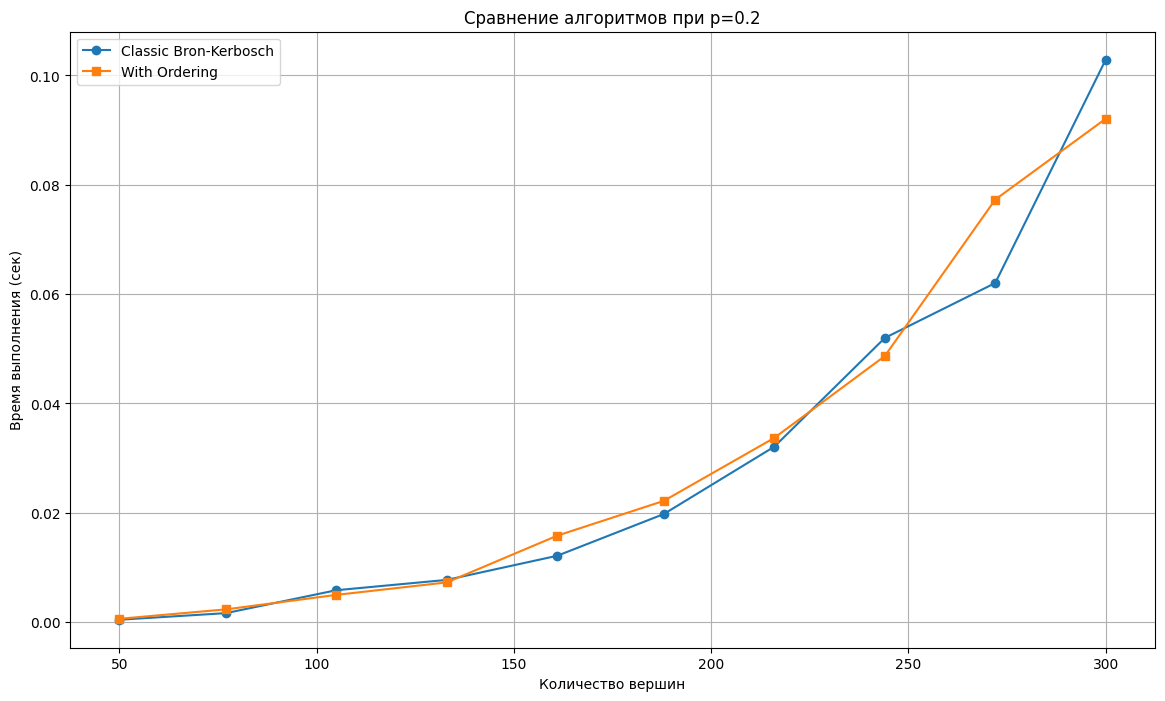
\includegraphics[width=0.7\textwidth]{image/rand1.png}
  \caption{p=0.2} % Подпись к первому изображению
  \label{fig:rand1} % Метка для ссылок на это изображение
\end{figure}

\begin{figure}[htbp]
  \centering
  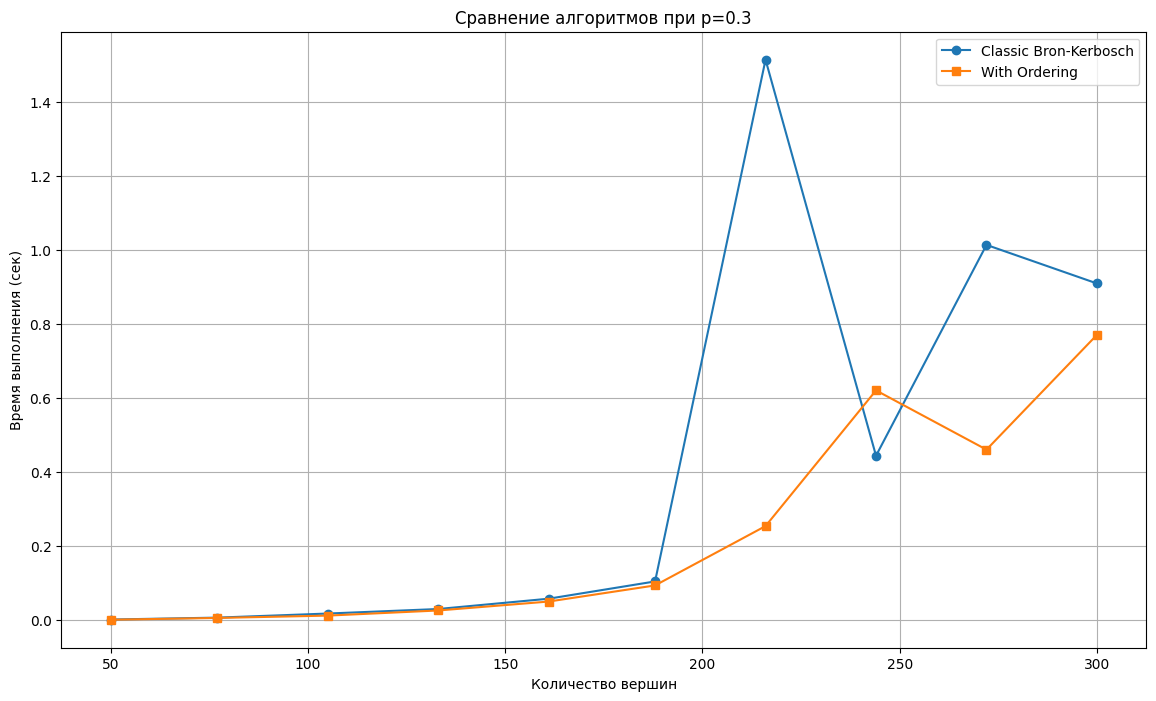
\includegraphics[width=0.7\textwidth]{image/rand2.png}
  \caption{p=0.3}
  \label{fig:rand2}
\end{figure}

\begin{figure}[htbp]
  \centering
  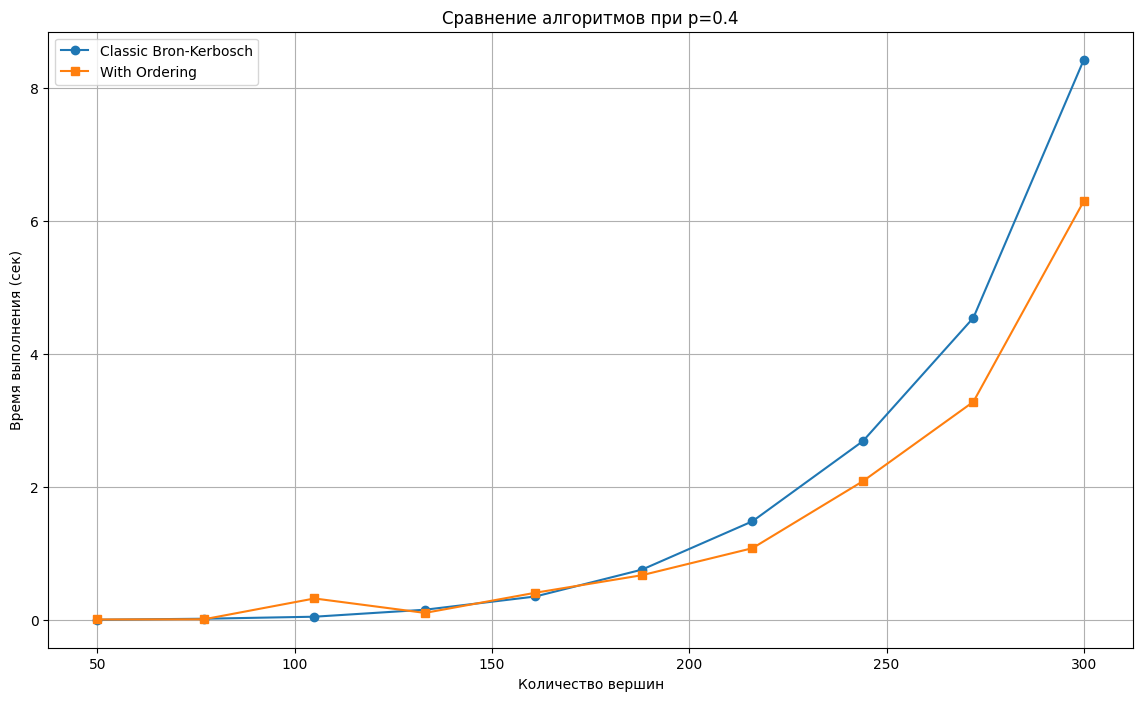
\includegraphics[width=0.7\textwidth]{image/rand3.png}
  \caption{p=0.4}
  \label{fig:rand3}
\end{figure}

Видим, что алгоритмы показывают себя практически одинаково. Связано это с тем, что вариант with ordering лучше всего показывает себя в случае большого числа немаксимальных клик, ожидать на случайных графах этого не стоит.

\subsection{Полные графы}
Рассмотрим полные графы с небольшим числом вершин (так как оригинальный алгоритм плохо справляется с такими графами) \ref{fig:rand4}
\begin{figure}[htbp]
  \centering
  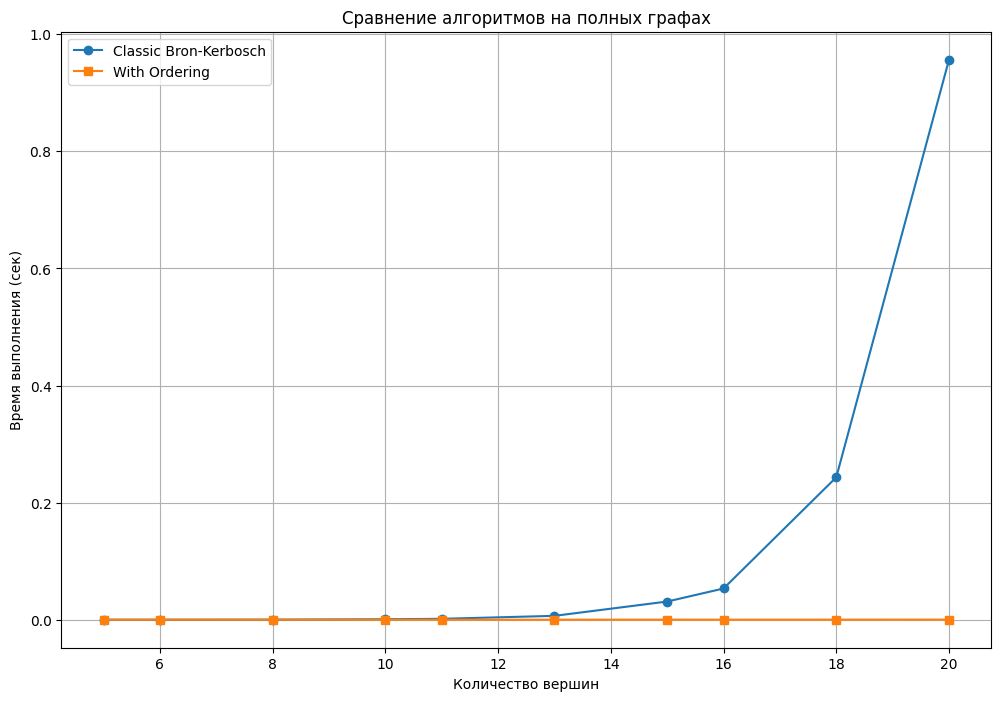
\includegraphics[width=0.7\textwidth]{image/complete_all.png}
  \caption{Сравнение алгоритмов на полных графах}
  \label{fig:rand4}
\end{figure}

Здесь мы видим главный недостаток исходного алгоритм. В то время как улучшенная версия отлично справляется (в полных графах только одна максимальная клика), оригинальный алгоритм перебирает все подмножества, из-за чего страдает.

\begin{figure}[htbp]
  \centering
  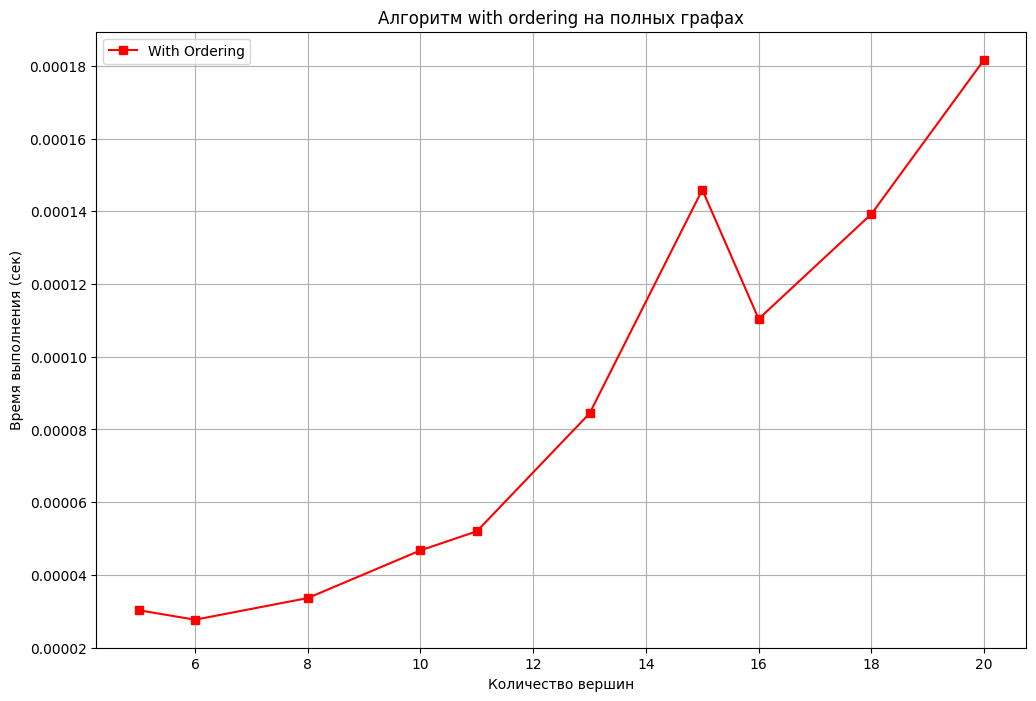
\includegraphics[width=0.7\textwidth]{image/complete_ord.png}
  \caption{Улучшенная версия алгоритма на полных графах}
  \label{fig:rand5}
\end{figure}

Видим, что время, затраченное улучшенной версией \ref{fig:rand5}, ничтожно.

\subsection{Графы Турана}
Рассматриваем графы Турана $T(n, \frac{n}{3})$ \ref{fig:rand6}.

\begin{figure}[htbp]
  \centering
  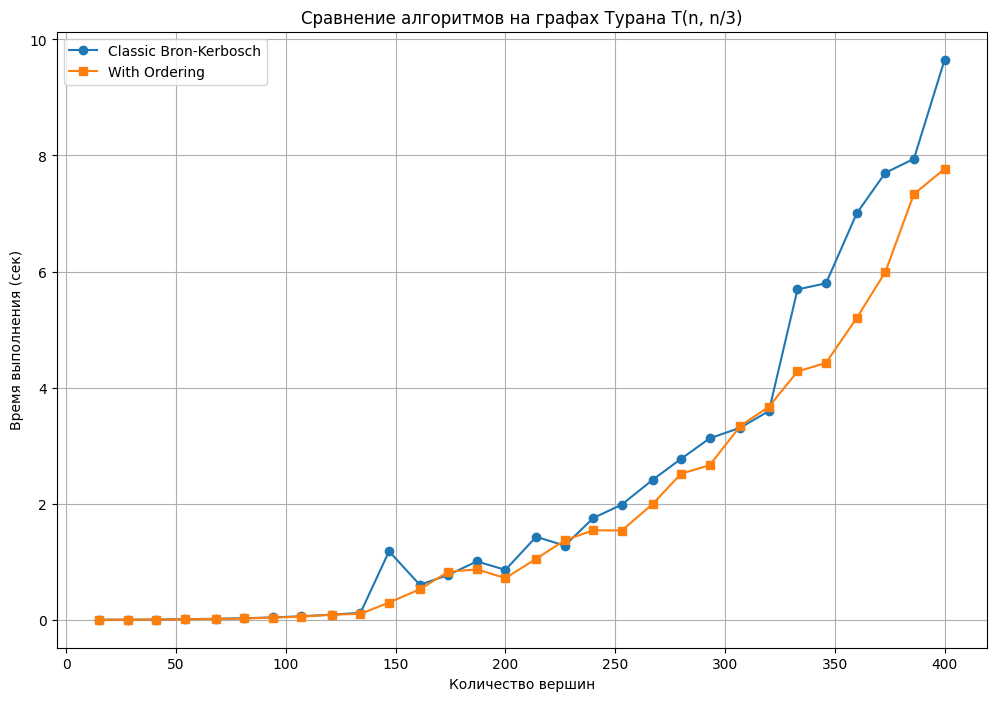
\includegraphics[width=0.7\textwidth]{image/turan.png}
  \caption{Сравнение алгоритмов на графах Турана}
  \label{fig:rand6}
\end{figure}
\newline
Видим, что в среднем улучшенная версия показывает себя лучше, но разрыв не настолько большой. Связано это с тем, что такие графы Турана - пример, когда наихудшая оценка на асимптотику достигается.
\newpage
\section{Вывод}
В работе мы рассмотрели задачу поиска максимальных клик в графе, а конкретно алгоритм Брона-Кербоша. Базовая версия может быть неэффективной на больших графах, поэтому расмотрели несколько стандартных его улучшений.

Первое улучшение — использование "поворотной вершины", которое позволяет избежать лишних проверок и ускорить поиск. Второе улучшение — это упорядочивание вершин, что позволяет минимизировать размер множества кандидатов на каждом шаге и таким образом уменьшить количество итераций.

На практике мы сравнили $2$ версии алгоритма на различных типах графов: случайных графах, полных графах и графах Турана. Эксперименты показали, что улучшенная версия, комбинирующая два улучшений работает в среднем быстрее, особенно быстрее на полных графах, где оригинальный алгоритм испытывает большие проблемы из-за перебора всех подмножеств.


\newpage

\begin{thebibliography}{9}

\bibitem{Tomita2006}
Etsuji Tomita, Akira Tanaka, and Haruhisa Takahashi.  
\textit{The worst-case time complexity for generating all maximal cliques and computational experiments}.  
The University of Electro-Communications, Department of Information and Communication Engineering, Chofu, Tokyo, Japan, 2006.

\bibitem{Bron1973}
Coen Bron and Joep Kerbosch.  
\textit{Algorithm 457: finding all cliques of an undirected graph}.  
Communications of the ACM, 1973.

\bibitem{Moon1965}
J.~W. Moon and L.~Moser.  
\textit{On cliques in graphs}.  
Israel Journal of Mathematics, 1965.

\end{thebibliography}
\end{document}